\mode<presentation>
{
  %\usetheme{umbc4}
  %\setbeamercovered{dynamic}
}
\usepackage[english]{babel}
% or whatever

\usepackage[latin1]{inputenc}
% or whatever

\usepackage{times}
\usepackage[T1]{fontenc}
% Or whatever. Note that the encoding and the font should match. If T1
% does not look nice, try deleting the line with the fontenc.
%--------------------------------------------------------------------------------------------
%--- Other packages
\usepackage{pstricks}
\usepackage{pst-node}
\usepackage{pst-rel-points}
\usepackage{xspace}

%%%%%% Declarations Defined in custom-foils
%\setfootline{\insertshortauthor, \insertshortinstitute \hfill   \insertshorttitle \hfill \insertframenumber/\inserttotalframenumber} 
\newcommand{\mypart}[1]{%
  \frame[plain]{\mbox{}\vfill \psshadowbox{\huge #1} \vfill\mbox{}}
}
\author[karkare]{Amey Karkare \\ \url{karkare@cse.iitk.ac.in}}
\date[]{\scalebox{0.3}{\includegraphics{iitklogo.epsi}}}%
\institute[CSE, IITK]{\url{http://www.cse.iitk.ac.in/~karkare/cs738}\\Department of CSE, IIT Kanpur}
\title[CS738]{CS738: Advanced Compiler Optimizations}
\subtitle[]{}


\subtitle[]{\ \\{\LARGE Data Flow Analysis}\\}
\newcommand{\bbent}{{\it Entry}\xspace}
\newcommand{\bbext}{{\it Exit}\xspace}

\newcommand{\IN}{{\sf IN}\xspace}
\newcommand{\OUT}{{\sf OUT}\xspace}

\newcommand{\Pred}{{\sf PRED}\xspace}
\newcommand{\Succ}{{\sf SUCC}\xspace}

\newcommand{\Kill}{{\sf KILL}\xspace}
\newcommand{\Gen}{{\sf GEN}\xspace}

\newcommand{\cmt}[1]{{}}
\newcommand{\meet}{\ensuremath{\bigwedge}\xspace}
\newcommand{\join}{\ensuremath{\bigvee}\xspace}
\newcommand{\glb}{{\sf glb}\xspace}
\newcommand{\lub}{{\sf lub}\xspace}

%% Framed minipage %%%%%%%%%%%%%%%%%%%%%%%%%%%%%%%%%%%%
\newsavebox\TestBox
\newenvironment{frmminipage}[2][]
{\begin{lrbox}{\TestBox}\begin{minipage}[#1]{#2}}
{\end{minipage}\end{lrbox}\fbox{\usebox{\TestBox}}}


\newcommand{\mylabbox}[2]{{\small #1}\psframebox{#2}\phantom{\small #1}}

\newcommand{\tossa}{%
  \ensuremath{\stackrel{SSA\quad\ }{\scalebox{3}{$\Rightarrow$}}}}

\newcommand{\jstfy}{\mbox{\phantom{XX}}}

\newcommand{\dom}{\operatorname{dom}}
\newcommand{\sdom}{\operatorname{sdom}}
\newcommand{\idom}{\operatorname{idom}}

\newcommand{\DOM}{\operatorname{DOM}}
\newcommand{\DF}{\operatorname{DF}}


\begin{document}

\frame{\titlepage}

\frame{
  \frametitle{Agenda}
  \begin{itemize}[<+->]
  \item Static analysis and compile-time optimizations
  \item For the next few lectures
  \item {\em Intraprocedural} Data Flow Analysis
    \begin{itemize}
    \item Classical Examples
    \item Components
    \end{itemize}
  \end{itemize}
}

\frame{
  \frametitle{Assumptions}
  \begin{itemize}[<+->]
  \item Intraprocedural: Restricted to a single function
  \item Input in 3-address format
  \item \alert{Unless otherwise specified}
  \end{itemize}
}

\frame{
  \frametitle{3-address Code Format}
  \begin{itemize}[<+->]
  \item Assignments
    \begin{itemize}
    \item[] x = y op z
    \item[] x = op y
    \item[] x = y
    \end{itemize}
  \item Jump/control transfer
    \begin{itemize}
    \item[] goto L
    \item[] if x relop y goto L
    \end{itemize}
  \item Statements can have label(s)
    \begin{itemize}
    \item[] L: \ldots
    \end{itemize}
  \item \alert{Arrays, Pointers and Functions to be added later when needed}
  \end{itemize}
}

\frame{
  \frametitle{Data Flow Analysis}
  \begin{itemize}[<+->]
  \item Class of techniques to derive information about flow of data
    \begin{itemize}
    \item along program execution paths
    \end{itemize}
  \item Used to answer questions such as:
    \begin{itemize}
    \item whether two identical expressions evaluate to same value
      \begin{itemize}
      \item used in common subexpression elimination
      \end{itemize}
    \item whether the result of an assignment is used later
      \begin{itemize}
      \item used by dead code elimination
      \end{itemize}
    \end{itemize}
  \end{itemize}
}

\frame{
  \frametitle{Data Flow Abstraction}
  \begin{itemize}[<+->]
  \item Basic Blocks (BB)
    \begin{itemize}
    \item sequence of 3-address code stmts
    \item single entry at the first statement 
    \item single exit at the last statement  
    \item Typically we use ``maximal'' basic block (maximal
      sequence of such instructions)
    \end{itemize}
  \end{itemize}
}

\frame{
  \frametitle{Identifying Basic Blocks}
  \begin{itemize}[<+->]
  \item {\em Leader}: The first statement of a basic block
    \begin{itemize}
    \item The first instruction of the program (procedure)
    \item Target of a branch (conditional and unconditional goto)
    \item Instruction immediately following a branch 
    \end{itemize}
  \end{itemize}
}

\frame{
  \frametitle{Special Basic Blocks}
  \begin{itemize}[<+->]
  \item Two special BBs are added to simplify the analysis
    \begin{itemize}
    \item empty (?) blocks!
    \end{itemize}
  \item \bbent: The first block to be executed for the procedure analyzed 
  \item \bbext: The last block to be executed 
  \end{itemize}
}

\frame{
  \frametitle{Data Flow Abstraction}
  \begin{itemize}[<+->]
  \item Control Flow Graph (CFG)
  \item A rooted directed graph $G = (N, E)$
  \item $N$ = set of BBs
    \begin{itemize}
    \item including  \bbent, \bbext
    \end{itemize}
  \item $E$ = set of edges
  \end{itemize}
}

\frame {
  \frametitle{CFG Edges}
  \begin{itemize}[<+->]
  \item Edge $B_1\rightarrow B_2 \in E$ if control can transfer from $B_1$ to $B_2$
    \begin{itemize}
    \item Fall through
    \item Through jump (goto)
    \item Edge from \bbent to (all?) real first BB(s)
    \item Edge to \bbext from all last BBs 
      \begin{itemize}
      \item BBs containing return
      \item Last real BB
      \end{itemize}
    \end{itemize}
  \end{itemize}
}

\frame{
  \frametitle{Data Flow Abstraction: Control Flow Graph}
  \begin{itemize}[<+->]
  \item Graph representation of paths that program may exercise
    during execution
  \item Typically one graph per procedure
  \item Graphs for separate procedures have to be
    combined/connected for interprocedural analysis
    \begin{itemize}
    \item Later!
    \item Single procedure, single flow graph for now.
    \end{itemize}
  \end{itemize}
}

\frame{
  \frametitle{Data Flow Abstraction: Program Points}
  \begin{itemize}[<+->]
  \item Input state/Output state for Stmt
    \begin{itemize}
    \item Program point before/after a stmt
    \item Denoted IN[s] and OUT[s]
    \item Within a basic block:
      \begin{itemize}
      \item Program point after a stmt is same as the program
        point before the next stmt
      \end{itemize}
    \end{itemize}
  \end{itemize}
}

\frame{
  \frametitle{Data Flow Abstraction: Program Points}
  \begin{itemize}[<+->]
  \item Input state/Output state for BBs
    \begin{itemize}
    \item Program point before/after a bb
    \item Denoted IN[$B$] and OUT[$B$]
    \item For  $B_1$ and $B_2$:
      \begin{itemize}
      \item if there is an edge from $B_1$ to $B_2$ in CFG, then
        the program point {\em after} the last stmt of $B_1$ {\em
          may be} followed immediately by the program point {\em
          before} the first stmt of $B_2$.
      \end{itemize}
    \end{itemize}
  \end{itemize}
}


\frame{
  \frametitle{Data Flow Abstraction: Execution Paths}
  \begin{itemize}[<+->]
  \item An execution path is of the form \[p_1, p_2, p_3,\ldots, p_n\]
  \item[] where $p_i \rightarrow p_{i+1}$ are adjacent program
    points in the CFG.
  \item Infinite number of possible execution paths in practical
    programs.
  \item Paths having no finite upper bound on the length.
  \item Need to {\em summarize} the information at a program
    point with a finite set of facts.
  \end{itemize}
}

\frame{
  \frametitle{Data Flow Schema}
  \begin{itemize}[<+->]
  \item Data flow values associated with each program point
    \begin{itemize}
    \item Summarize all possible states at that point
    \end{itemize}
  \item {\em Domain:} set of all possible data flow values
  \item Different domains for different analyses/optimizations
  \end{itemize}
}

\frame{
  \frametitle{Data Flow Problem}
  \begin{itemize}[<+->]
  \item Constraints on data flow values
    \begin{itemize}
    \item Transfer constraints
    \item Control flow constraints
    \end{itemize}
  \item {\bf Aim:} To find a solution to the constraints
    \begin{itemize}
    \item Multiple solutions possible 
    \item Trivial solutions, \ldots, Exact solutions
    \end{itemize}
  \item We typically compute approximate solution
    \begin{itemize}
    \item Close to the exact solution (as close as possible!)
    \item Why not exact solution?
    \end{itemize}
  \end{itemize}
}

\frame{
  \frametitle{Data Flow Constraints: Transfer Constraints}
  \begin{itemize}[<+->]
  \item Transfer functions
    \begin{itemize}
    \item relationship between the data flow values before and after a stmt
    \end{itemize}
  \item forward functions: Compute facts {\em after} a statement
    $s$ from the facts available {\em before} $s$.
    \begin{itemize}
    \item General form:
      \[ \OUT[s] = f_s(\IN[s]) \]
    \end{itemize}
  \item backward functions: Compute facts {\em before} a statement
    $s$ from the facts available {\em after} $s$.
    \begin{itemize}
    \item General form:
      \[ \IN[s] = f_s(\OUT[s]) \]
    \end{itemize}
  \item $f_s$ depends on the statement and the analysis
  \end{itemize}
}
\frame{
  \frametitle{Data Flow Constraints: Control Flow Constraints}
  \begin{itemize}[<+->]
  \item Relationship between the data flow values of two points that are related by program execution semantics
  \item For a basic block having $n$ statements:
    \[\IN[s_{i+1}] = \OUT[s_i], i = 1,2,\ldots,n-1\]
  \item $\IN[s_1]$,  $\OUT[s_n]$ to come later
  \end{itemize}
}

\newcommand{\Comb}{\ensuremath{\bigoplus}}
\frame{
  \frametitle{Data Flow Constraints: Notations}
  \begin{itemize}[<+->]
  \item \Pred(B): Set of predecessor BBs of block $B$ in CFG
  \item \Succ(B): Set of successor BBs of block $B$ in CFG
  \item $f \circ g$ : Composition of functions $f$ and $g$
  \item \Comb: An abstract operator denoting some way of combining
    facts present in a set .
  \end{itemize}
}
\frame{
  \frametitle{Data Flow Constraints: Basic Blocks}
  \begin{itemize}[<+->]
  \item {\bf Forward}
    \begin{itemize}
    \item For $B$ consisting of $s_1, s_2, \ldots, s_n$
      \[f_B = f_{s_n} \circ \ldots \circ f_{s_2} \circ f_{s_1}\]
      \[\OUT[B] = f_B(\IN[B])\]
    \item Control flow constraints
      \[\IN[B] = \Comb_{P \in \Pred(B)} \OUT[P]\]
    \end{itemize}
  \item {\bf Backward}
    \[f_B = f_{s_1} \circ f_{s_2} \circ \ldots \circ f_{s_n}\] 
    \[ \IN[B] = f_B(OUT[B]) \]
    \[ \OUT[B] = \Comb_{S \in \Succ(B)} IN[S] \]
  \end{itemize}
}

\frame{
  \frametitle{Data Flow Equations}
  \begin{itemize}[<+->]
  \item Typical Equation
    \[ \OUT[s] = \IN[s] - kill[s] \cup gen[s] \]
  \item[] $gen(s)$: information generated
  \item[] $kill(s)$: information killed
  \item Example:\\
    {\tt \begin{tabular}{rcll}
        a &=& b*c   &
        {\color{red!80} // generates expression b * c} \\
        c &=& 5       &
        {\color{red!80} // kills expression b*c}  \\
        d &=& b*c   &
        {\color{red!80} // is b*c redundant here?} 
    \end{tabular}}
  \end{itemize}
}

\frame{
  \frametitle{Example Data Flow Analysis}
  \begin{itemize}
  \item Reaching Definitions Analysis
  \item Definition of a variable $x$:
    $x = \ldots {\sf something} \ldots$
  \item Could be more complex (e.g. through pointers, references,
    implicit)

  \end{itemize}
}
\frame{
  \frametitle{Reaching Definitions Analysis}
  \begin{itemize}
  \item A definition $d$ reaches a point $p$ if
    \begin{itemize}
    \item there is a path from the point {\em immediately
      following} $d$ to $p$
    \item $d$ is not ``killed'' along that path
    \item ``Kill'' means redefinition of the left hand side ($x$
      in the earlier example)
    \end{itemize}
  \end{itemize}
}

\frame{
  \frametitle{RD Analysis of a Structured Program}
  \begin{center}
    \psset{unit=1mm}
    \begin{pspicture}(0,0)(50,30)
      %\psframe(0,0)(50,30)
      \putnode{s1}{origin}{25}{15}{%
        \psovalbox[fillstyle=solid,fillcolor=lightgray]{$d: x = y + z$}}
      \putnode{se}{s1}{0}{15}{}
      \putnode{sx}{s1}{0}{-15}{}
      \putnode{sl}{s1}{20}{0}{$s_1$}
      \ncline{->}{se}{s1}\Aput{$\IN(s_1)$}
      \ncline{->}{s1}{sx}\Aput{$\OUT(s_1)$}
    \end{pspicture}\pause
    \begin{eqnarray*}
      \OUT(s_1) &=& \IN(s_1) - \Kill(s_1) \cup \Gen(s_1)\\ \pause
      \Gen(s_1) &=& \pause \{d\} \\ \pause
      \Kill(s_1) &=& \pause D_x - \{d\}, \mbox{where $D_x$: set of all definitions of $x$}\\ \pause
      \Kill(s_1) &=& \pause D_x \mbox{?\pause\ \ will also work here}\\
      && \qquad\mbox{but may not work in general}
    \end{eqnarray*}
  \end{center}
}

\frame{
  \frametitle{RD Analysis of a Structured Program}
  \begin{center}
    \psset{unit=1mm}
    \begin{pspicture}(0,0)(50,30)
      \psframe[fillstyle=solid, fillcolor=blue!20](5,5)(45,25)
      \putnode{se}{origin}{25}{29}{}
      \putnode{s1}{se}{0}{-10}{%
        \psovalbox[fillstyle=solid,fillcolor=lightgray]{$s_1$}}
      \putnode{s2}{s1}{0}{-10}{%
        \psovalbox[fillstyle=solid,fillcolor=lightgray]{$s_2$}}
      \putnode{sx}{s2}{0}{-10}{}
      \putnode{lbl}{origin}{43}{23}{$S$}
      \ncline{->}{se}{s1}\aput[0.2](.1){{\small$\IN(S)$}}
      \ncline{->}{s1}{s2}
      \ncline{->}{s2}{sx}\aput[0.2](.6){{\small$\OUT(S)$}}
    \end{pspicture}\pause
    \begin{eqnarray*}
      \Gen(S) &=& \pause \Gen(s_1) - \Kill(s_2) \cup \Gen(s_2) \\ \pause
      \Kill(S) &=& \pause \Kill(s_1) - \Gen(s_2) \cup \Kill(s_2)\\ \pause
      \IN(s_1) &=& \pause \IN(S) \\ \pause
      \IN(s_2) &=& \pause \OUT(s_1) \\ \pause
      \OUT(S) &=& \pause \OUT(s_2)
    \end{eqnarray*}
  \end{center}
}


\frame{
  \frametitle{RD Analysis of a Structured Program}
  \begin{center}
    \psset{unit=1mm}
    \begin{pspicture}(0,0)(50,30)
      \psframe[fillstyle=solid, fillcolor=blue!20](5,5)(45,25)
      \putnode{se}{origin}{25}{29}{}
      \putnode{see}{se}{0}{-7}{}
      \putnode{s1}{see}{-10}{-8}{%
        \psovalbox[fillstyle=solid,fillcolor=lightgray]{$s_1$}}
      \putnode{s2}{s1}{20}{0}{%
        \psovalbox[fillstyle=solid,fillcolor=lightgray]{$s_2$}}
      \putnode{sxx}{s2}{-10}{-8}{}
      \putnode{sx}{sxx}{0}{-7}{}
      \putnode{lbl}{origin}{43}{23}{$S$}
      \ncline{-}{se}{see}\aput[0.2](.1){{\small$\IN(S)$}}
      \ncline[nodesepB=-1.1]{->}{see}{s1}
      \ncline[nodesepB=-1.1]{->}{see}{s2}
      \ncline[nodesepA=-1.1]{-}{s1}{sxx}
      \ncline[nodesepA=-1.1]{-}{s2}{sxx}      
      \ncline{->}{sxx}{sx}\aput[0.2](.6){{\small$\OUT(S)$}}
    \end{pspicture}\pause
    \begin{eqnarray*}
      \Gen(S) &=& \pause \Gen(s_1) \cup \Gen(s_2) \\ \pause
      \Kill(S) &=& \pause \Kill(s_1) \cap \Kill(s_2)\\ \pause
      \IN(s_1) &=& \pause \IN(s_2) \quad = \quad \IN(S) \\ \pause
      \OUT(S) &=& \pause \OUT(s_1) \cup \OUT(s_2)
    \end{eqnarray*}
  \end{center}
}

\frame{
  \frametitle{RD Analysis of a Structured Program}
  \begin{center}
    \psset{unit=1mm}
    \begin{pspicture}(0,0)(50,30)
      \psframe[fillstyle=solid, fillcolor=blue!20](5,5)(45,25)
      \putnode{s1}{origin}{25}{15}{%
        \psovalbox[fillstyle=solid,fillcolor=lightgray]{$s_1$}}
      \putnode{se}{s1}{0}{15}{}
      \putnode{sx}{s1}{0}{-15}{}
      \putnode{lbl}{origin}{43}{23}{$S$}
      \ncline{->}{se}{s1}\aput(0.2){$\IN(S)$}
      \ncline{->}{s1}{sx}\aput(0.8){$\OUT(S)$}
      \nccurve[angleA=-135,angleB=135,ncurv=4,nodesep=-1.0]{->}{s1}{s1}
    \end{pspicture}\pause
    \begin{eqnarray*}
      \Gen(S) &=& \pause \Gen(s_1) \\ \pause
      \Kill(S) &=& \pause \Kill(s_1) \\ \pause
      \OUT(S) &=& \pause \OUT(s_1) \\ \pause
      \IN(s_1) &=& \pause \IN(S) \cup \Gen(s_1)
    \end{eqnarray*}
  \end{center}
}


\frame{
  \frametitle{RD Analysis is Approximate}
  \begin{center}
    \psset{unit=1mm}
    \begin{pspicture}(0,0)(50,30)
      \psframe[fillstyle=solid, fillcolor=blue!20](5,5)(45,25)
      \putnode{se}{origin}{25}{29}{}
      \putnode{see}{se}{0}{-7}{}
      \putnode{s1}{see}{-10}{-8}{%
        \psovalbox[fillstyle=solid,fillcolor=lightgray]{$s_1$}}
      \putnode{s2}{s1}{20}{0}{%
        \psovalbox[fillstyle=solid,fillcolor=lightgray]{$s_2$}}
      \putnode{sxx}{s2}{-10}{-8}{}
      \putnode{sx}{sxx}{0}{-7}{}
      \putnode{lbl}{origin}{43}{23}{$S$}
      \ncline{-}{se}{see}\aput[0.2](.1){{\small$\IN(S)$}}
      \ncline[nodesepB=-1.1]{->}{see}{s1}
      \ncline[nodesepB=-1.1]{->}{see}{s2}
      \ncline[nodesepA=-1.1]{-}{s1}{sxx}
      \ncline[nodesepA=-1.1]{-}{s2}{sxx}      
      \ncline{->}{sxx}{sx}\aput[0.2](.6){{\small$\OUT(S)$}}
    \end{pspicture}%\pause
    \begin{itemize}[<+->]
    \item Assumption: All paths are feasible.
    \item Example: 
    {\tt \begin{tabbing}
        if (true) \= s1; \\
        else      \> s2;
    \end{tabbing}}\pause
    $\begin{array}{rclcl}
      {\bf Fact} & & {\bf Computed} && {\bf Actual} \\
      \Gen(S)  &=& \Gen(s_1) \cup \Gen(s_2)   &\supseteq& \Gen(s_1) \\ \pause
      \Kill(S) &=& \Kill(s_1) \cap \Kill(s_2) &\subseteq& \Kill(s_1)\\
    \end{array}$
    \end{itemize}
  \end{center}
}

\frame{
  \frametitle{RD Analysis is Approximate}
  \begin{center}
    \psset{unit=1mm}
    \begin{pspicture}(0,0)(50,30)
      \psframe[fillstyle=solid, fillcolor=blue!20](5,5)(45,25)
      \putnode{se}{origin}{25}{29}{}
      \putnode{see}{se}{0}{-7}{}
      \putnode{s1}{see}{-10}{-8}{%
        \psovalbox[fillstyle=solid,fillcolor=lightgray]{$s_1$}}
      \putnode{s2}{s1}{20}{0}{%
        \psovalbox[fillstyle=solid,fillcolor=lightgray]{$s_2$}}
      \putnode{sxx}{s2}{-10}{-8}{}
      \putnode{sx}{sxx}{0}{-7}{}
      \putnode{lbl}{origin}{43}{23}{$S$}
      \ncline{-}{se}{see}\aput[0.2](.1){{\small$\IN(S)$}}
      \ncline[nodesepB=-1.1]{->}{see}{s1}
      \ncline[nodesepB=-1.1]{->}{see}{s2}
      \ncline[nodesepA=-1.1]{-}{s1}{sxx}
      \ncline[nodesepA=-1.1]{-}{s2}{sxx}      
      \ncline{->}{sxx}{sx}\aput[0.2](.6){{\small$\OUT(S)$}}
    \end{pspicture}%\pause
    \begin{itemize}[<+->]
    \item Thus,
      \begin{itemize}
      \item[] true $\Gen(S) \subseteq$ analysis $\Gen(S)$
      \item[] true $\Kill(S) \supseteq$ analysis $\Kill(S)$
      \end{itemize}
    \item More definitions computed to be reaching than actually do!
    \item Later we shall see that this is {\red SAFE} approximation
      \begin{itemize}
      \item prevents optimizations
      \item but NO wrong optimization
      \end{itemize}
    \end{itemize}
  \end{center}
}

\frame{
  \frametitle{RD at BB level}
  \begin{itemize}[<+->]
  \item A definition $d$ can reach the start of a block from any of
    its predecessor
    \begin{itemize}
    \item if it reaches the end of some predecessor
    \end{itemize}
    \[\IN(B) = \bigcup_{P\in\Pred(B)} \OUT(P)\]
  \item A definition $d$ reaches the end of a block if
    \begin{itemize}
    \item either it is generated in the block
    \item or it reaches block and not killed
    \end{itemize}
    \[ \OUT(B) = \IN(B) - \Kill(B) \cup \Gen(B) \]
  \end{itemize}
}

\frame{
  \frametitle{Solving RD Constraints}
  \begin{itemize}[<+->]
  \item \Kill \& \Gen  known for each BB.
  \item A program with $N$ BBs has $2N$ equations with $2N$
    unknowns.
    \begin{itemize}
    \item Solution is possible.
    \item Iterative approach (on the next slide).
    \end{itemize}
  \end{itemize}
}

\frame{
  \frametitle{}\vspace{2cm}
  \small\tt
  \begin{tabbing}
    for \=each block $B$ \{\\ \pause
    \> $\OUT(B) = \emptyset;$\\ \pause
    \} \\
       {\bf $\OUT(\bbent) = \emptyset;$}
       {\red // note this for later discussion}\\ \pause
    change = true;\\
    while (change) \{\\
    \>change = false;\\ \pause
    \>for \=each block $B$ other than $\bbent$ \{\\ \pause
    \>\>$\IN(B) = \bigcup_{P \in \Pred(B)}\OUT(P);$\\ \pause
    \>\>oldOut = $\OUT(B)$;\\
    \>\>$\OUT(B) = \IN(B) - \Kill(B) \cup \Gen(B);$\\ \pause
    \>\>if (\=$\OUT(B) \not= $oldOut) then \{\\
    \>\>\>  change = true;\\
    \>\>\}\\
    \>\}\\
    \}
  \end{tabbing}
}

\frame{
  \frametitle{Reaching Definitions: Example}
  \begin{minipage}{.4\textwidth}
  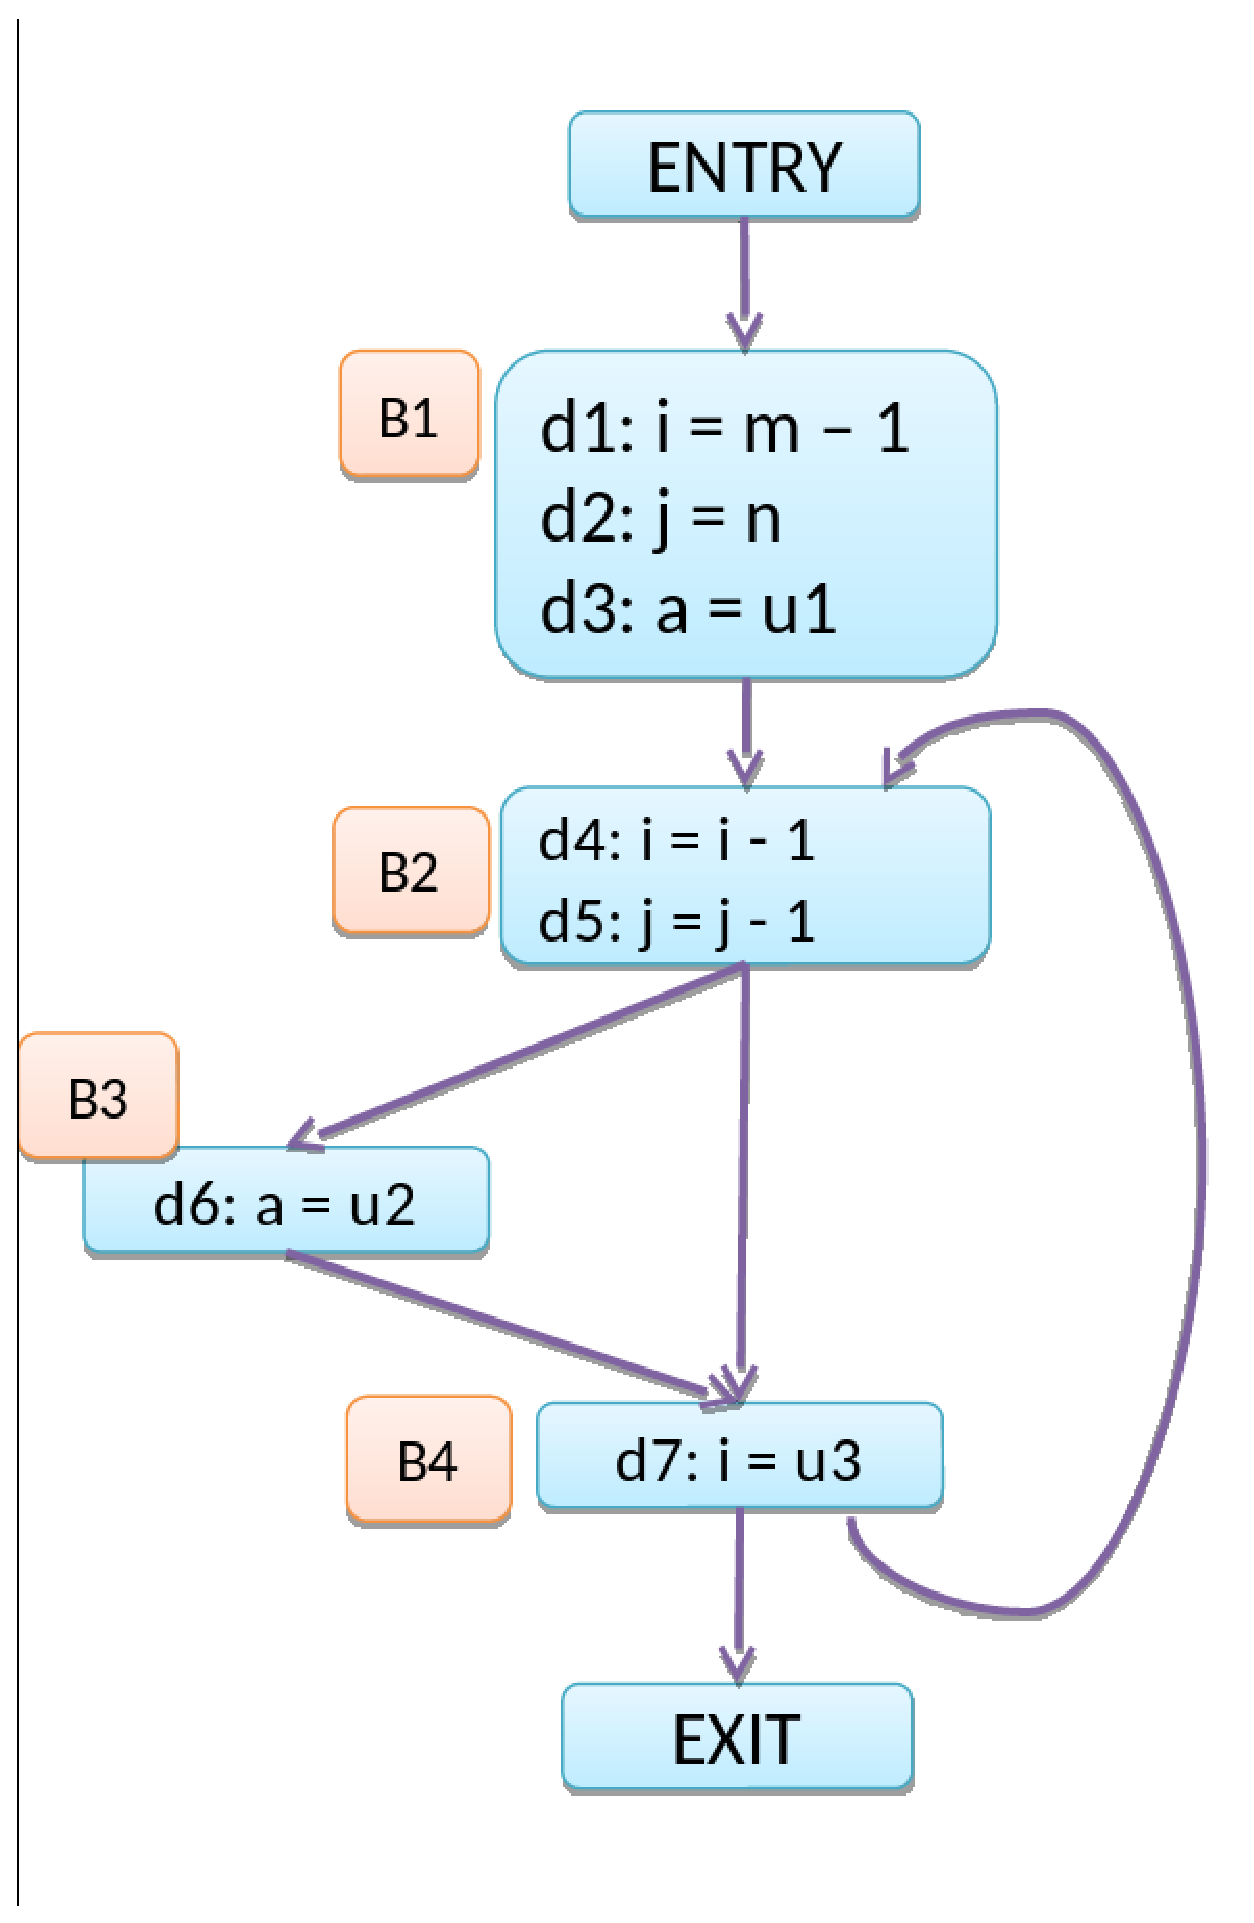
\includegraphics[width=120bp]{RD_Examp.eps}    
  \end{minipage}\pause
  \begin{minipage}{.45\textwidth}
  \begin{tabular}[t]{|c|c|c|}
    \hline
        {\bf BB} & {\bf \Gen}     & {\bf \Kill} \\ \hline \hline
        B1       & \only<3->{\{d1, d2, d3\}} & \only<4->{\{d4, d5, d6, d7\}} \\ \hline 
        B2       & \only<5->{\{d4, d5\}}     & \only<6->{\{d1, d2, d7\}} \\ \hline 
        B3       & \only<7->{\{d6\}}         & \only<8->{\{d3\}} \\ \hline 
        B4       & \only<9->{\{d7\}}         & \only<10>{\{d1, d4\}} \\ \hline 
  \end{tabular}
  \end{minipage}
}

\frame{
  \frametitle{Reaching Definitions: Example}
  \begin{minipage}{.4\textwidth}
  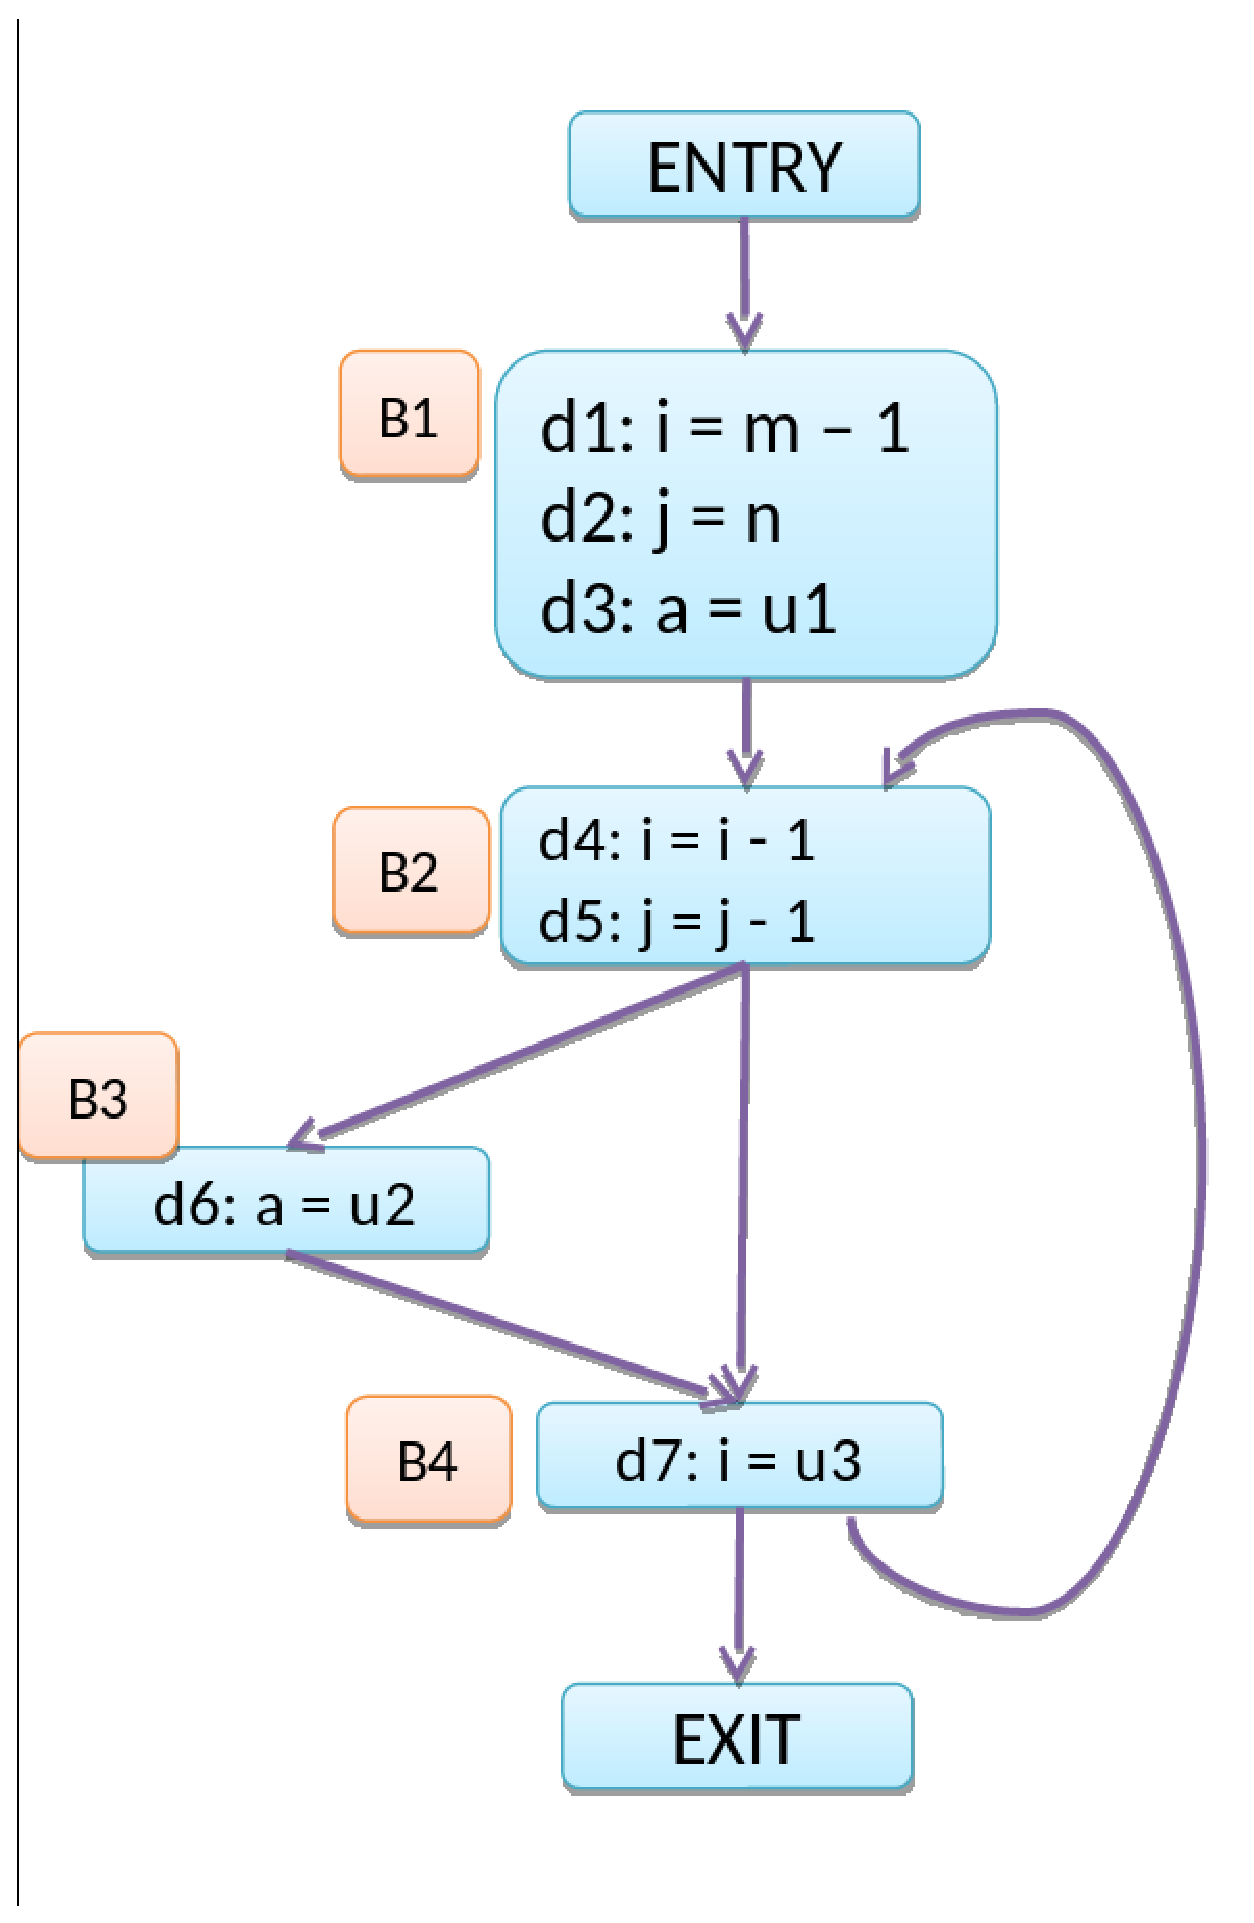
\includegraphics[width=120bp]{RD_Examp.eps}    
  \end{minipage}
  \begin{minipage}{.45\textwidth}\scriptsize
  \begin{tabular}[t]{|@{}c@{}|@{}c@{\ }||p{8mm}|p{9mm}|p{8mm}|p{8mm}|}
    \hline
        {\bf Pass\#} & {\bf Pt} & {\bf B1} & {\bf B2} & {\bf B3} & {\bf B4}
        \\ \hline \hline
        Init & \IN  & - & - & - & -  \\ \cline{2-6} 
        & \OUT & $\emptyset$ & $\emptyset$ & $\emptyset$ & $\emptyset$ \\\hline
        \pause
        1 & \IN & $\emptyset$ & d1, d2, d3 & d3, d4, d5 & d3, d4, d5, d6 \\ \cline{2-6}
        & \OUT & d1, d2, d3 & d3, d4, d5& d4, d5, d6 & d3, d5, d6, d7 \\ \hline
        \pause
        2 & \IN & $\emptyset$ & d1, d2, d3, d5, d6, d7&d3, d4, d5, d6&d3, d4, d5, d6 \\ \cline{2-6}
        &\OUT & d1, d2, d3& d3, d4, d5, d6 & d4, d5, d6& d3, d5, d6, d7 \\ \hline 
        \pause
        3 & \IN & $\emptyset$ & d1, d2, d3, d5, d6, d7 & d3, d4, d5, d6&d3, d4, d5, d6 \\ \cline{2-6} 
        &\OUT & d1, d2, d3& d3, d4, d5, d6& d4, d5, d6 & d3, d5, d6, d7 \\ \hline 
  \end{tabular}
  \end{minipage}
}

\frame{
  \frametitle{Reaching Definitions: Bitvectors}
  \begin{minipage}{.4\textwidth}
  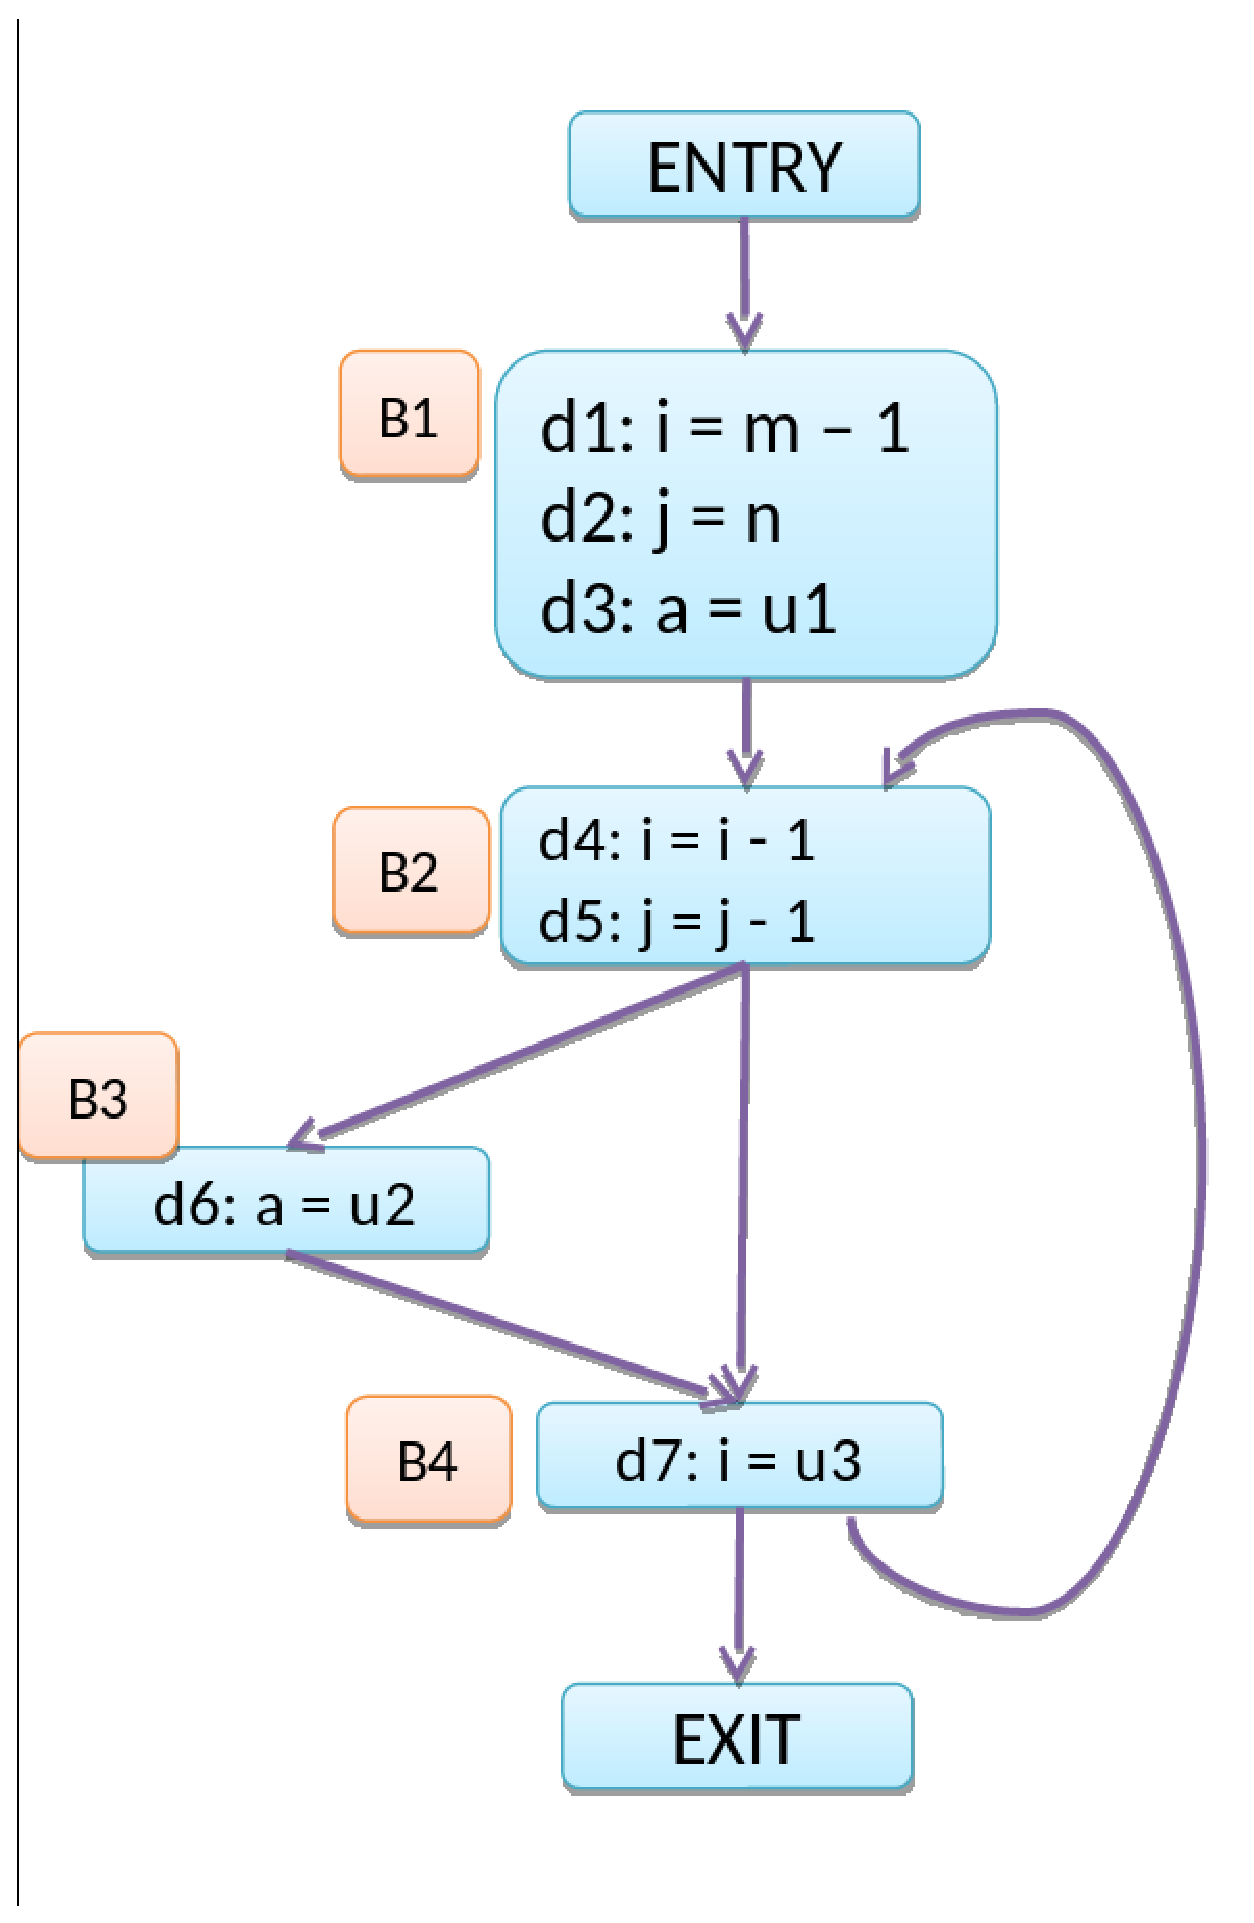
\includegraphics[width=120bp]{RD_Examp.eps}    
  \end{minipage}
  \begin{minipage}{.45\textwidth}\scriptsize
    a bit for each definition: \\
    \begin{tabular}{|@{\ }c@{\ }|@{\ }c@{\ }|@{\ }c@{\ }|@{\ }c@{\ }|@{\ }c@{\ }|@{\ }c@{\ }|@{\ }c@{\ }|}
      \hline d1 & d2 & d3 & d4 & d5 & d6 & d7 \\ \hline
    \end{tabular} \pause
    
  \begin{tabular}[t]{|@{}c@{}|@{}c@{\ }||@{\ }c@{\ }|@{\ }c@{\ }|@{\ }c@{\ }|@{\ }c@{\ }|}
    \hline
        {\bf Pass\#} & {\bf Pt} & {\bf B1} & {\bf B2} & {\bf B3} & {\bf B4}
        \\ \hline \hline
        Init & \IN  & - & - & - & -  \\ \cline{2-6} 
        & \OUT & 0000000 & 0000000 & 0000000 & 0000000 \\\hline
        1 & \IN & 0000000 & 1110000 & 0011100 & 0011110 \\ \cline{2-6}
        & \OUT & 1110000 & 0011100 & 0001110 & 0010111 \\ \hline
        2 & \IN & 0000000 & 1110111&0011110&0011110 \\ \cline{2-6}
        &\OUT & 1110000& 0011110 & 0001110& 0010111 \\ \hline 
        3 & \IN & 0000000 & 1110111 & 0011110&0011110 \\ \cline{2-6} 
        &\OUT & 1110000& 0011110& 0001110 & 0010111 \\ \hline 
  \end{tabular}
  \end{minipage}
}

\frame{
  \frametitle{Reaching Definitions: Bitvectors}
  \begin{itemize}[<+->]
  \item Set-theoretic  definitions:
    \[\IN(B) = \bigcup_{P\in\Pred(B)} \OUT(P)\]
    \[ \OUT(B) = \IN(B) - \Kill(B) \cup \Gen(B) \]
  \item Bitvector definitions:
    \[\IN(B) = \bigvee_{P\in\Pred(B)} \OUT(P)\]
    \[ \OUT(B) = \IN(B) \wedge \neg\Kill(B) \vee \Gen(B) \]
  \item Bitwise $\vee, \wedge, \neg$ operators
  \end{itemize}
}

\frame{
  \frametitle{Reaching Definitions: Application}
  \begin{center}
    {\bf Constant Folding}
  \end{center}\tt
  \begin{tabbing}
    whi\=le changes occur \{ \\ \pause
    \>for\= all the stmts S of the program \{ \\ \pause
    \>\>for\= each operand B of S \{ \\ \pause
    \>\>\>if \=there is a unique definition of B   \\
    \>\>\>that reaches S and is a constant C  \{ \\  \pause
    \>\>\>\>replace B by C in S; \\ \pause
    \>\>\>\>if \=all operands of S are constant \{\\ \pause
    \>\>\>\>\>replace rhs by eval(rhs); \\ \pause
    \>\>\>\>\>mark definition as constant; \\
    \}\}\}\}\}
  \end{tabbing}
}

\frame{
  \frametitle{Reaching Definitions: Application}
  \begin{itemize}[<+->]
  \item Recall the approximation in reaching definition analysis
    \begin{itemize}
    \item[] true $\Gen(S) \subseteq$ analysis $\Gen(S)$
    \item[] true $\Kill(S) \supseteq$ analysis $\Kill(S)$
    \end{itemize}
  \item Can it cause the application to infer
    \begin{itemize}
    \item an expression as a constant when it is has different
      values for different executions?
    \item an expression as not a constant when it is a constant
      for all executions?
    \end{itemize}
  \item Safety? Profitability?
  \end{itemize}
}

\frame{
  \frametitle{Reaching Definitions: Summary}
  \begin{itemize}[<+->]
  \item $\Gen(B) = \left\{ d_x\ \begin{array}{|l}d_x \mbox{ in $B$ defines variable $x$ and is not} \\ \mbox{followed by another definition of $x$ in $B$}
  \end{array}\right\}$
  \item $\Kill(B) = \{ d_x \mid \mbox{$B$ contains some definition of $x$ }\}$
  \item $\IN(B) = \bigcup_{P\in\Pred(B)} \OUT(P)$
  \item $\OUT(B) = \IN(B) - \Kill(B) \cup \Gen(B)$
  \item meet ( $\bigwedge$ ) operator: The operator to combine information coming along different predecessors is $\cup$
  \item \alert{What about the \bbent block?}
  \end{itemize}
}

\frame{
  \frametitle{Reaching Definitions: Summary}
  \begin{itemize}[<+->]
  \item Entry block has to be initialized specially:
    \begin{eqnarray*}
      \OUT(\bbent) &=& {\sf Entry Info}\\
          {\sf Entry Info}&=& \emptyset
    \end{eqnarray*}
  \item A better entry info could be:
    \begin{eqnarray*}
      {\sf Entry Info} &=& \{ x = undefined \mid x\ is\ a\ variable\}
    \end{eqnarray*}
  \item Why?
  \end{itemize}
}

\end{document}
